\documentclass[11pt,a4paper]{ctexart}
\usepackage{geometry}
\geometry{margin=2.2cm}
\usepackage{amsmath,amssymb}
\usepackage{booktabs}
\usepackage{siunitx}
\usepackage{graphicx}
\usepackage{array}
\usepackage[hypertexnames=false]{hyperref}
\usepackage{float}
\usepackage{enumitem}
\usepackage{longtable}
\usepackage{xcolor}
\setlength{\emergencystretch}{8em}

\hypersetup{
  colorlinks=true,
  linkcolor=blue!50!black,
  urlcolor=blue!50!black,
  citecolor=blue!50!black
}

\title{2D 双目标首达问题中的数值方法比较报告\\
\large C1 场景：Sparse Exact / Dense Recursion / AW(Cauchy-FFT) / Giuggioli Defect-Reduced AW / 线性方程}
\author{valley-k-small: \texttt{reports/2d\_two\_target\_double\_peak}}
\date{2026-02-10}

\begin{document}
\sloppy
\maketitle

\begin{abstract}
本报告针对 \texttt{2d\_two\_target\_double\_peak} 的 C1 配置，系统比较五类数值方法在同一模型上的精度、效率和适用性：
\textbf{(1) 时间域 sparse exact 递推}、
\textbf{(2) 显式 transient 矩阵的 dense recursion}、
\textbf{(3) Luca/Giuggioli 缺陷降阶反演（Method C）}、
\textbf{(4) 全量 AW/Cauchy-FFT 反演（Method C0，对照）}、
\textbf{(5) 线性方程法（MFPT/splitting）}。
结果显示：分布层面 sparse 与 dense 在机器精度内一致；AW 与 defect-reduced AW 在同一时间窗内与 exact 高精一致；但 MFPT 对长尾高度敏感，截断求和会显著低估，线性方程法最稳健。
\end{abstract}

\section{问题与模型设置}
\subsection{目标}
比较以下三个维度：
\begin{enumerate}[leftmargin=2em]
  \item \textbf{FPT 分布精度}：是否能准确恢复双峰结构与峰位；
  \item \textbf{MFPT 稳健性}：是否受截断尾部影响；
  \item \textbf{计算效率}：在本规模下的 wall-clock 代价。
\end{enumerate}

\subsection{统一实验配置（C1）}
\begin{itemize}[leftmargin=2em]
  \item 网格：$N=31$，四边反射；
  \item 基础运动：$q=0.2$（移动），$1-q=0.8$（停留）；
  \item 局部偏置：$\delta=0.2$，从 stay 概率中抽取并加到箭头方向；
  \item 起点：$n_0=(14,14)$（0-based）；
  \item 目标：$m_1=(21,14),\ m_2=(6,6)$（0-based）；
  \item 主时域上限：$t_{\max}=6000$，停止阈值 $S(t)<10^{-13}$；
  \item AW 窗口：$t_{\max}^{\mathrm{AW}}=800$，oversample$=2$，$r\_\text{pow10}=8.0$，对应 $m=2048$。
\end{itemize}

\section{统一数学框架（详细原理）}
\subsection{吸收马尔可夫链分块}
将状态分为 transient 集 $\mathcal T$ 与吸收集 $\mathcal A=\{m_1,m_2\}$，转移矩阵写成
\[
P=
\begin{pmatrix}
Q & R\\
0 & I
\end{pmatrix},\qquad
R=[r_1\ r_2].
\]
其中 $Q\in\mathbb R^{|\mathcal T|\times|\mathcal T|}$，$r_1,r_2\in\mathbb R^{|\mathcal T|}$。
起点分布记为行向量 $\alpha$（one-hot）。

\subsection{FPT、survival、MFPT 的统一公式}
定义 $u_t=\alpha Q^t$（第 $t$ 步仍在 transient 子空间的分布），则
\[
f_1(t)=\alpha Q^{t-1}r_1,\quad
f_2(t)=\alpha Q^{t-1}r_2,\quad
f_{\mathrm{any}}(t)=f_1(t)+f_2(t).
\]
\[
S(t)=\Pr(T>t)=u_t\mathbf 1=\alpha Q^t\mathbf 1.
\]
离散时间下：
\[
f_{\mathrm{any}}(t)=S(t-1)-S(t),\qquad
\mathbb E[T]=\sum_{t\ge 0}S(t).
\]
这说明 MFPT 对长尾特别敏感，是后续截断误差的根本原因。

\section{五类方法与流程}
\subsection{方法 A：Sparse exact 时间迭代（当前主脚本方法）}
该方法在概率空间直接递推（脚本里对应“每步摘除目标概率”）：
\begin{enumerate}[leftmargin=2em]
  \item 在全状态空间推进一步概率；
  \item 读取本步落在 $m_1,m_2$ 的概率质量，得到 $f_1(t),f_2(t)$；
  \item 将 $m_1,m_2$ 位置概率清零后继续推进；
  \item 得 $f_{\mathrm{any}}(t)=f_1(t)+f_2(t)$ 与 $S(t)$。
\end{enumerate}
其数学等价形式是对 $u_t$ 做递推：
\[
u_t=u_{t-1}Q,\quad f_i(t)=u_{t-1}r_i.
\]
若按边列表（稀疏）更新，单步代价是 $\mathcal O(E)$（$E$ 为有效转移边数），总时间
\[
\mathcal O(t_{\max}E),\qquad \text{内存 } \mathcal O(N).
\]
该方法天然给出整条 FPT 曲线，双峰诊断最直接；但 MFPT 截断误差显著依赖尾部长度。

\subsection{方法 B：Dense recursion（transient 子空间）}
把两目标设为吸收，构造
\[
Q\in\mathbb{R}^{|\mathcal T|\times |\mathcal T|},\quad r_1,r_2\in\mathbb{R}^{|\mathcal T|},\quad u_0=\alpha,
\]
然后递推
\[
u_t=u_{t-1}Q,\quad f_i(t)=u_{t-1}r_i,\quad f_{\mathrm{any}}(t)=f_1(t)+f_2(t).
\]
它与方法 A 数学等价，但数值实现上显式持有 dense $Q$。
若 $n_T:=|\mathcal T|$，单步向量-矩阵乘法是 $\mathcal O(n_T^2)$，总时间
\[
\mathcal O(t_{\max}n_T^2),\qquad \text{内存 } \mathcal O(n_T^2).
\]
因此它更适合作为正确性基线，而不是大规模主算法。

\subsection{方法 C：Luca/Giuggioli 缺陷降阶反演（已实现）}
这一节给出本项目实际使用的 Luca 方法数学流程。

\textbf{步骤 C1：缺陷分解。}
把 transient 算子写成
\[
Q=Q_0+\sum_{e=1}^{M}\delta_e\,\mathbf e_{u_e}\mathbf e_{v_e}^{\top}
=Q_0+U\Delta V^\top,
\]
其中 $Q_0$ 是可解基底，$M$ 是 defect pair 数，$\Delta=\mathrm{diag}(\delta_1,\dots,\delta_M)$。

\textbf{步骤 C2：用 Woodbury 只恢复所需传播子。}
对复点 $z$，先定义
\[
P^0(z):=(I-zQ_0)^{-1}.
\]
只取需要的节点集合 $S=\{s,m_1,m_2\}$ 与 $T=\{m_1,m_2\}$，有
\[
P_{S,T}(z)
=P^0_{S,T}(z)
+z\,P^0_{S,U}(z)\,\Delta
\bigl[I_M-z\,P^0_{V,U}(z)\,\Delta\bigr]^{-1}
P^0_{V,T}(z).
\]
这样每个 $z_k$ 的主要求解从 $n_T\times n_T$ 变成 $M\times M$。

\textbf{步骤 C3：两目标 renewal 闭合。}
由实现里使用的两目标关系，
\[
\begin{bmatrix}
P_{s,m_1}(z)\\
P_{s,m_2}(z)
\end{bmatrix}
=
\begin{bmatrix}
P_{m_1,m_1}(z) & P_{m_2,m_1}(z)\\
P_{m_1,m_2}(z) & P_{m_2,m_2}(z)
\end{bmatrix}
\begin{bmatrix}
F_1(z)\\
F_2(z)
\end{bmatrix},
\]
因此每个 $z$ 只需再解一个 $2\times2$ 系统 $F(z)=G(z)^{-1}b(z)$。

\textbf{步骤 C4：Cauchy-FFT 反演回时域。}
\[
 f_i(t)\approx r^{-t}\cdot\frac{1}{m}\sum_{k=0}^{m-1}F_i(z_k)e^{-i2\pi kt/m}.
\]

对应复杂度：
\[
\mathcal O\!\big(m\,[C_{\text{base}}(n_T)+M^3]+m\log m\big),
\]
其中 $C_{\text{base}}(n_T)$ 是基底 Green 项在所需节点上的求值开销。
本项目已在 C1 上实装并基准该方法。

\subsection{方法 C0：全量 AW / Cauchy-FFT（对照基线）}
作为对照，full AW 直接计算
\[
\tilde f_i(z)=z\,\alpha\,(I-zQ)^{-1}r_i,
\]
每个 $z_k$ 需要一次完整 $n_T\times n_T$ 复数线性求解，总复杂度
\[
\mathcal O(m\,n_T^3 + m\log m),\qquad \text{内存 } \mathcal O(n_T^2+m).
\]
本报告中 full AW 仍只在 $t\le 800$ 时间窗上用于对照。

\subsection{方法 D：线性方程（MFPT / splitting）}
仅求矩而非整条分布：
\[
(I-Q)m=\mathbf 1,\qquad (I-Q)u_i=r_i.
\]
起点分量给出
\[
\mathrm{MFPT}=m(n_0),\quad p_i=u_i(n_0),\quad p_1+p_2=1.
\]
若采用 dense direct solve，三次求解总代价约
\[
\mathcal O(n_T^3),\qquad \text{内存 } \mathcal O(n_T^2).
\]
若改用稀疏迭代，可降到“每次迭代 $\mathcal O(E)$，迭代次数依条件数而定”。该方法对长尾最稳健。

\section{复杂度总表（统一口径）}
\begin{table}[H]
  \centering
  \small
  \begin{tabular}{>{\raggedright\arraybackslash}p{3.1cm}>{\raggedright\arraybackslash}p{5.3cm}>{\raggedright\arraybackslash}p{3.8cm}}
    \toprule
    方法 & 时间复杂度（主导项） & 内存复杂度 \\
    \midrule
    Sparse exact 递推 & $\mathcal O(t_{\max}E)$ & $\mathcal O(N)$ \\
    Dense recursion ($Q$) & $\mathcal O(t_{\max}n_T^2)$ & $\mathcal O(n_T^2)$ \\
    Luca/Giuggioli 缺陷降阶（Method C） & $\mathcal O(m[C_{\text{base}}(n_T)+M^3]+m\log m)$ & $\mathcal O(M^2+n_T)$ 到 $\mathcal O(n_T^2)$ \\
    全量 AW/Cauchy-FFT（Method C0） & $\mathcal O(m\,n_T^3+m\log m)$（dense solve） & $\mathcal O(n_T^2+m)$ \\
    线性方程（MFPT/splitting） & $\mathcal O(n_T^3)$（dense solve） & $\mathcal O(n_T^2)$ \\
    \bottomrule
  \end{tabular}
  \caption{复杂度估计汇总。符号：$N$=总状态数，$E$=有效边数，$n_T=|\mathcal T|$，$m$=反演采样点，$M$=缺陷维度。}
\end{table}

\subsection{本 C1 场景的量级代入}
本实验实际规模为
\[
N=31^2=961,\quad n_T=959,\quad E\approx 4681,\quad m=2048.
\]
据此可直观看到：
\begin{itemize}[leftmargin=2em]
  \item Sparse exact 的主代价约随 $t_{\max}\times 4.7\times 10^3$ 线性增长；
  \item Dense recursion 随 $t_{\max}\times 9.2\times 10^5$ 量级增长；
  \item 全量 AW（Method C0）含约 $m$ 次完整复数线性求解，成本远高于前两者；
  \item C1 的 defect 规模（本实现）为
  \[
  M_{\text{pairs}}=632,\quad M_{\text{nodes}}=326,\quad M_{\text{local-bias-sites}}=317;
  \]
  \item 若按 pair 维度（$M=632$）估算，求解核降幅约
  \[
  (n_T/M)^3=(959/632)^3\approx 3.5\times
  \]
  （若用 $2.81$ 指数，则约 $(959/632)^{2.81}\approx 3.2\times$）；
  \item 线性方程法只需少量系统求解，因此在“只关心 MFPT/splitting”时最划算。
\end{itemize}

\subsection{与文献复杂度记号的对应}
为避免口径混淆，这里统一说明：格点文献中的 $N^d$ 对应状态空间量级（本报告中可类比为 $n_T$），
$M$ 则是 defect 表示下的缺陷维度。Sarvaharman--Giuggioli（Phys.\ Rev.\ Research 5, 013118，Sec.\ V）
给出的口径是：显式首达公式约为 $\mathcal O(M^2N^d)$，暴力时间迭代约为 $\mathcal O(N^{2d}t)$；
同段也提到若采用更快矩阵乘法指数可写成 $2.373d$。一些旧文中出现的 $2.81$ 是 Strassen 风格指数假设。
因此“$2.81$ vs $2.373$”的差异来自线性代数模型假设，而不是方法结构矛盾。

\section{实测结果}
\subsection{运行时间}
\begin{table}[H]
  \centering
  \begin{tabular}{lc}
    \toprule
    方法 & 运行时间 (s) \\
    \midrule
    Sparse exact 递推 & 0.0561 \\
    Dense recursion (Q) & 0.0919 \\
    Luca/Giuggioli 缺陷降阶（Method C） & 78.0223 \\
    全量 AW/Cauchy 反演（Method C0） & 47.2622 \\
    线性方程 (MFPT/splitting) & 0.0213 \\
    \bottomrule
  \end{tabular}
  \caption{C1 场景下五类方法的 wall-clock 对比。}
\end{table}

\subsection{分布误差（以 sparse exact 为基准）}
\begin{table}[H]
  \centering
  \begin{tabular}{lcc}
    \toprule
    对比项 & $L^1$ 误差 & $L^\infty$ 误差 \\
    \midrule
    Dense vs Sparse（共同步长） & $9.212\times 10^{-15}$ & $1.924\times 10^{-18}$ \\
    Luca-defect（C）vs Sparse（$1..t_{\max}^{\mathrm{AW}}$） & $9.912\times 10^{-10}$ & $1.426\times 10^{-12}$ \\
    Full AW（C0）vs Sparse（$1..t_{\max}^{\mathrm{AW}}$） & $9.912\times 10^{-10}$ & $1.426\times 10^{-12}$ \\
    \bottomrule
  \end{tabular}
  \caption{分布层面对比：dense 与 sparse 在机器精度内一致；两条变换域路线在同窗都高精。}
\end{table}

\subsection{关键统计量}
\begin{table}[H]
  \centering
  \small
  \begin{tabular}{lcccccc}
    \toprule
    方法 & mass\_any & tail & MFPT(截断/精确) & peak1 & peak2 \\
    \midrule
    Sparse exact（$t\le 6000$） & 0.850786 & 0.149214 & 1583.479 & 35 & 284 \\
    Sparse exact（$t\le 800$） & 0.297030 & 0.702970 & 111.653 & 35 & 284 \\
    Dense recursion（$t\le 6000$） & 0.850786 & 0.149214 & 1583.479 & 35 & 284 \\
    Luca defect-reduced（$t\le 800$） & 0.297030 & 0.702970 & 111.653 & 35 & 284 \\
    Full AW inversion（$t\le 800$） & 0.297030 & 0.702970 & 111.653 & 35 & 284 \\
    线性方程（全时域） & 1.000000 & 0.000000 & 3011.214 & - & - \\
    \bottomrule
  \end{tabular}
  \caption{Luca-defect 与 Full AW 行都与 ``Sparse exact（$t\le800$）'' 一致，说明本窗反演精度可靠。}
\end{table}

\subsection{Defect 规模与实测影响（C1）}
\begin{itemize}[leftmargin=2em]
  \item 本实现的 defect 规模：local-bias sites $=317$，defect pairs $=632$，defect nodes $=326$。
  \item 实测结果：Luca-defect（Method C）用时 $78.0$s，慢于 Full AW 基线（Method C0）的 $47.3$s。
  \item 原因：在该 defect 规模下，求解核降阶收益不足以抵消基底 Green 函数求值与矩阵装配开销。
  \item 启示：当 defect 支撑更稀疏（$M\ll n_T$）或进一步压缩 defect 维度时，降阶路线更可能出现速度优势。
\end{itemize}

\subsection{MFPT 截断偏差（长尾效应）}
\begin{table}[H]
  \centering
  \small
  \begin{tabular}{ccccc}
    \toprule
    $t_{\max}$ & 吸收质量 & 尾部质量 & MFPT 截断值 & 相对误差（对线性方程） \\
    \midrule
    300 & 0.116714 & 0.883286 & 19.294 & -99.359\% \\
    600 & 0.241807 & 0.758193 & 73.099 & -97.572\% \\
    1200 & 0.389579 & 0.610421 & 203.559 & -93.240\% \\
    2400 & 0.581766 & 0.418234 & 540.034 & -82.066\% \\
    6000 & 0.850786 & 0.149214 & 1583.479 & -47.414\% \\
    \bottomrule
  \end{tabular}
  \caption{MFPT 明显由长尾主导，截断会系统性低估。}
\end{table}

\subsection{构造的 Luca 最快案例（LF1）}
为回答“Luca 何时会比所有对照更快”，我们构造了一个超稀疏缺陷案例（单一 local-bias 点）并实测全部方法：
\[
N=41,\quad n_T=1679,\quad t_{\max}=12000,\quad t_{\max}^{\mathrm{AW}}=80,\quad M_{\text{pairs}}=2.
\]
\begin{table}[H]
  \centering
  \begin{tabular}{lc}
    \toprule
    方法 & 运行时间 (s) \\
    \midrule
    Luca/Giuggioli 缺陷降阶（Method C） & 0.0198 \\
    线性方程 (MFPT/splitting) & 0.0477 \\
    Sparse exact 递推 & 0.1754 \\
    Dense recursion (Q) & 1.6187 \\
    全量 AW/Cauchy（Method C0） & 22.8746 \\
    \bottomrule
  \end{tabular}
  \caption{LF1 构造案例：Luca 方法在该参数区间最快。}
\end{table}
\begin{figure}[H]
  \centering
  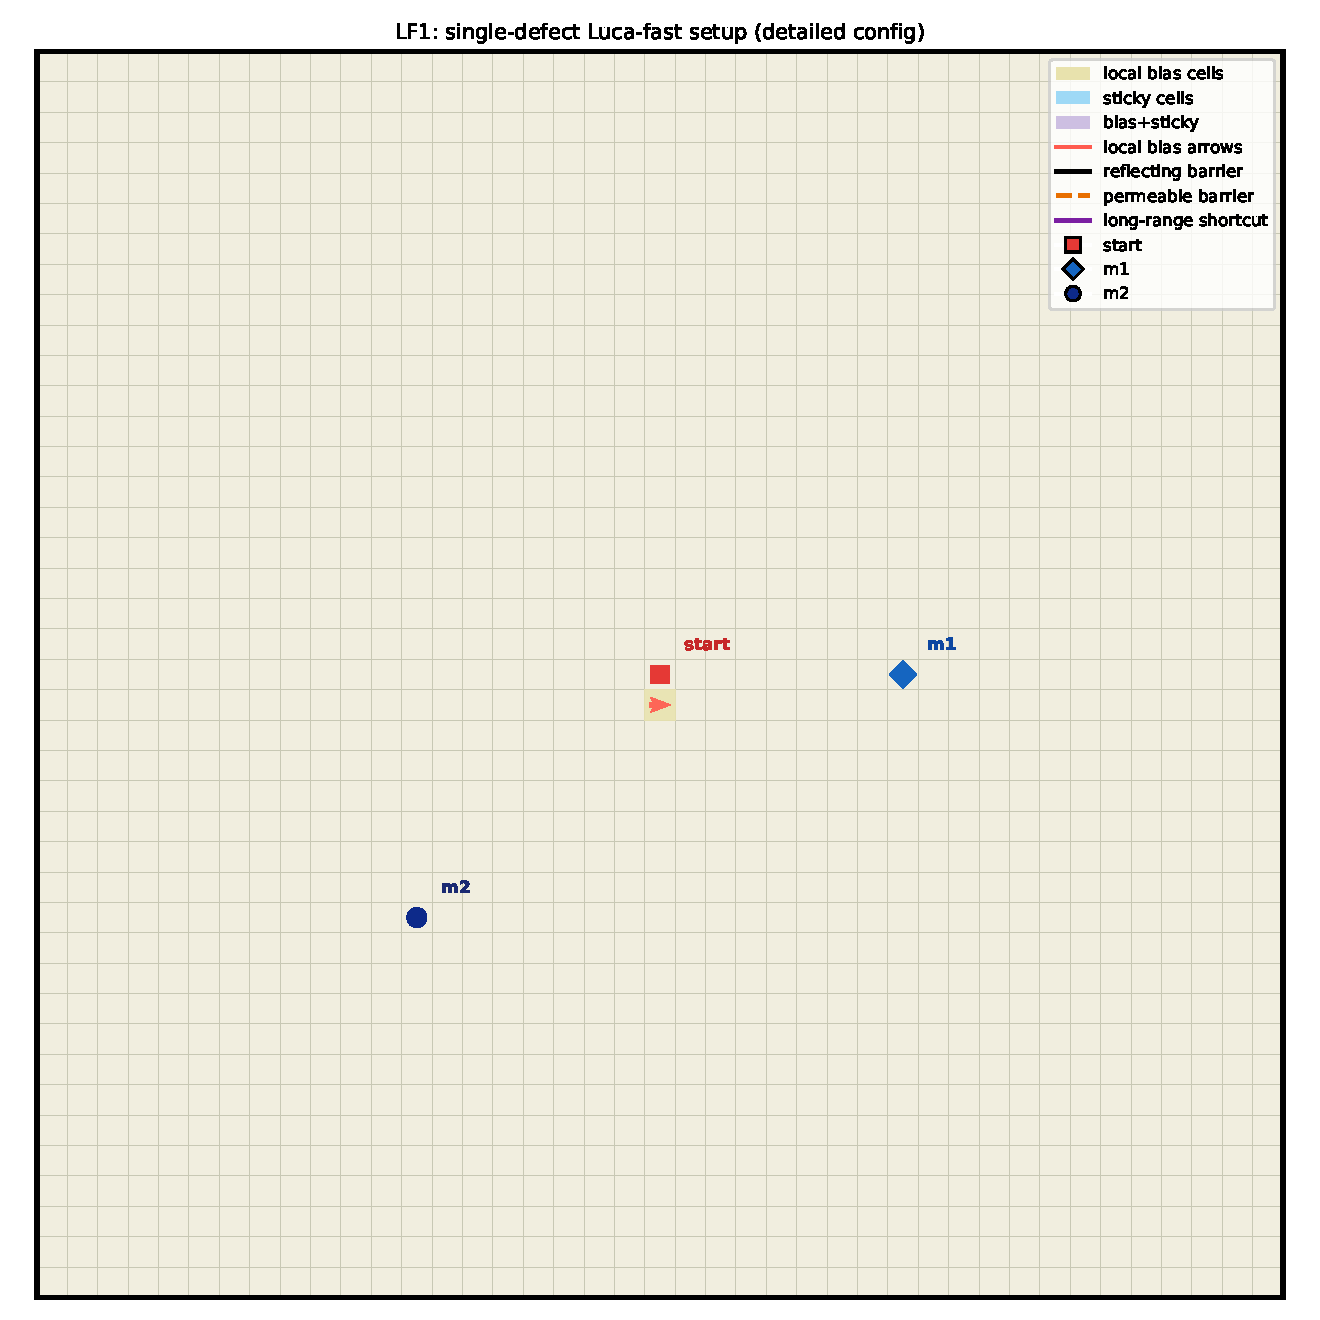
\includegraphics[width=0.78\linewidth]{figures/luca_fast_case_config_detailed.pdf}
  \caption{LF1 配置图（与同目录 external detailed config 相同绘图风格）。}
\end{figure}
\begin{figure}[H]
  \centering
  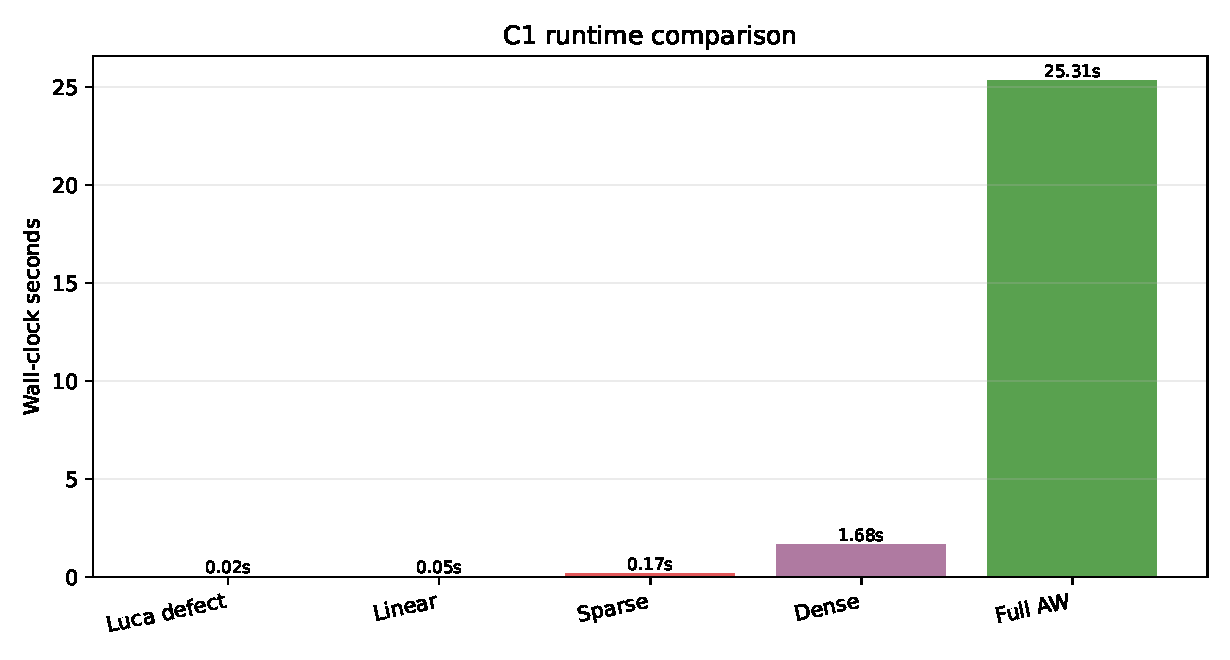
\includegraphics[width=0.88\linewidth]{figures/luca_fast_case_runtime.pdf}
  \caption{LF1 运行时间对比。}
\end{figure}
LF1 的关键原因是缺陷维度极小（$M=2$）使得 Method C 的缺陷求解几乎退化为常数规模，而 full AW 与 dense 路线仍需处理大规模线性代数核心。

\section{图形对照}
\begin{figure}[H]
  \centering
  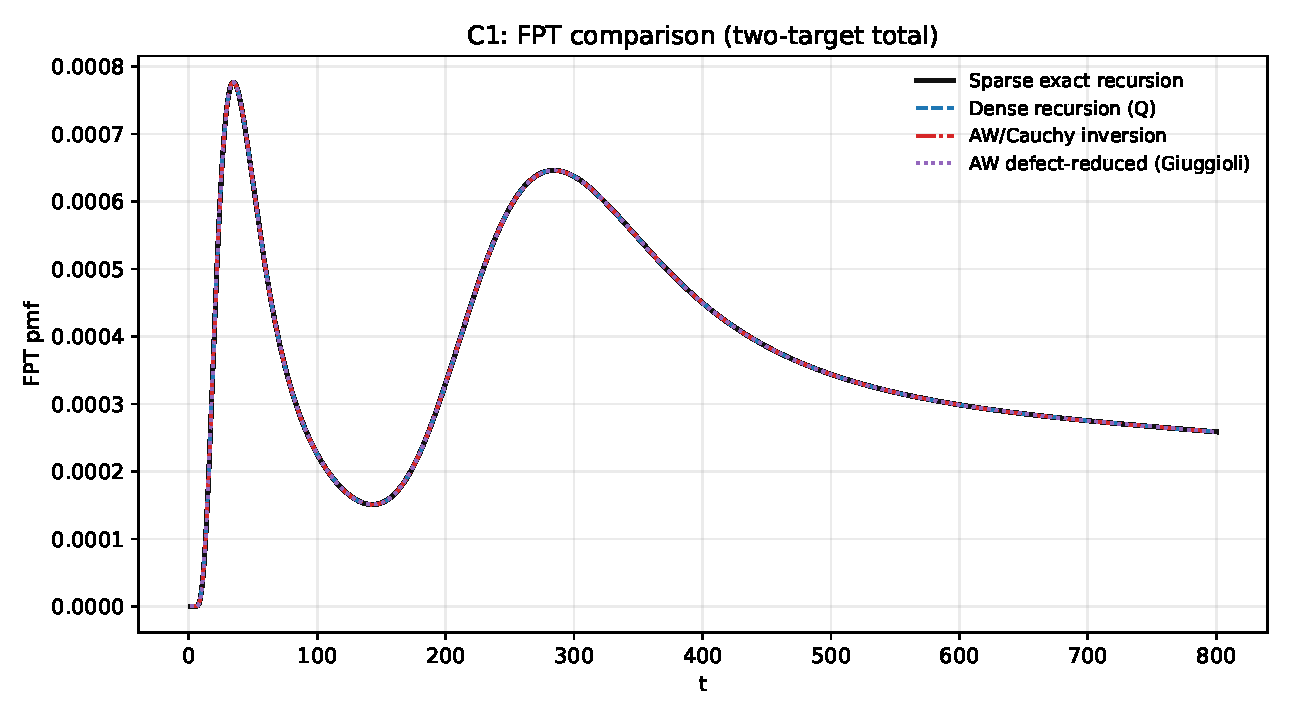
\includegraphics[width=0.95\linewidth]{figures/method_compare_c1_fpt_overlay.pdf}
  \caption{FPT 曲线叠加：Sparse / Dense / Luca-defect / Full AW（在同窗几乎重合）。}
\end{figure}

\begin{figure}[H]
  \centering
  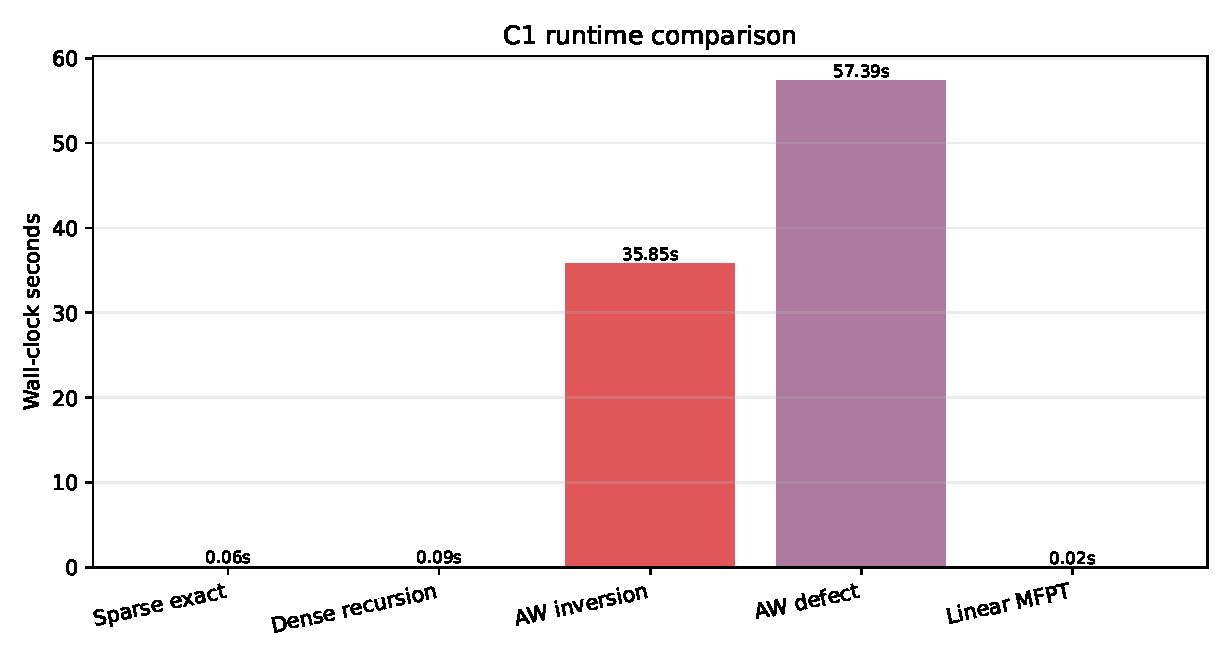
\includegraphics[width=0.88\linewidth]{figures/method_compare_c1_runtime.pdf}
  \caption{运行时间对比。}
\end{figure}

\section{结论与建议}
\begin{enumerate}[leftmargin=2em]
  \item \textbf{要整条双峰曲线}：优先 sparse exact（快、直接、稳定）。
  \item \textbf{要稳健 MFPT/splitting}：优先线性方程法，不要依赖截断求和。
  \item \textbf{Method C（Luca）}：数学机制清晰且分布精度高；但在本 C1 defect 规模下速度不占优。
  \item \textbf{要做变换域分析}：可先用 Full AW（Method C0）作基线；当 $M\ll n_T$ 且实现开销可控时，优先 Method C。
\end{enumerate}

\section*{复现}
\begin{verbatim}
cd reports/grid2d_two_target_double_peak
.venv/bin/python code/compare_numeric_methods.py
\end{verbatim}

\end{document}
